\documentclass{article}
\usepackage{listings}
\usepackage{mathrsfs}
\usepackage[utf8]{inputenc}
\usepackage{amssymb}
\usepackage{lipsum}
\usepackage{amsmath}
\usepackage{fancyhdr}
\usepackage{geometry}
\usepackage{scrextend}
\usepackage[english,german]{babel}
\usepackage{titling}
\setlength{\droptitle}{-3cm}
\usepackage{tikz}
\usepackage{algorithm,algpseudocode}
\usepackage[doublespacing]{setspace}
\usetikzlibrary{datavisualization}
\usetikzlibrary{datavisualization.formats.functions}
\usepackage{polynom}
\usepackage{amsmath}
\usepackage{gauss}
\usepackage{tkz-euclide}
\usetikzlibrary{datavisualization}
\usetikzlibrary{datavisualization.formats.functions}
\author{
Alexander Mattick Kennung: qi69dube\\
Kapitel 1
}
\usepackage{import}
\date{\today}
\geometry{a4paper, margin=2cm}
\usepackage{stackengine}
\parskip 1em
\newcommand\stackequal[2]{%
  \mathrel{\stackunder[2pt]{\stackon[4pt]{=}{$\scriptscriptstyle#1$}}{%
  $\scriptscriptstyle#2$}}
 }
\makeatletter
\renewcommand*\env@matrix[1][*\c@MaxMatrixCols c]{%
  \hskip -\arraycolsep
  \let\@ifnextchar\new@ifnextchar
  \array{#1}}
\makeatother
\lstset{
  language=haskell,
}
\lstnewenvironment{code}{\lstset{language=Haskell,basicstyle=\small}}{}
\usepackage{enumitem}
\setlist{nosep}
\usepackage{titlesec}

\titlespacing*{\subsection}{0pt}{2pt}{3pt}
\titlespacing*{\section}{0pt}{0pt}{5pt}
\titlespacing*{\subsubsection}{0pt}{1pt}{2pt}
\title{Vorlesung 4}


\begin{document}
	\maketitle
	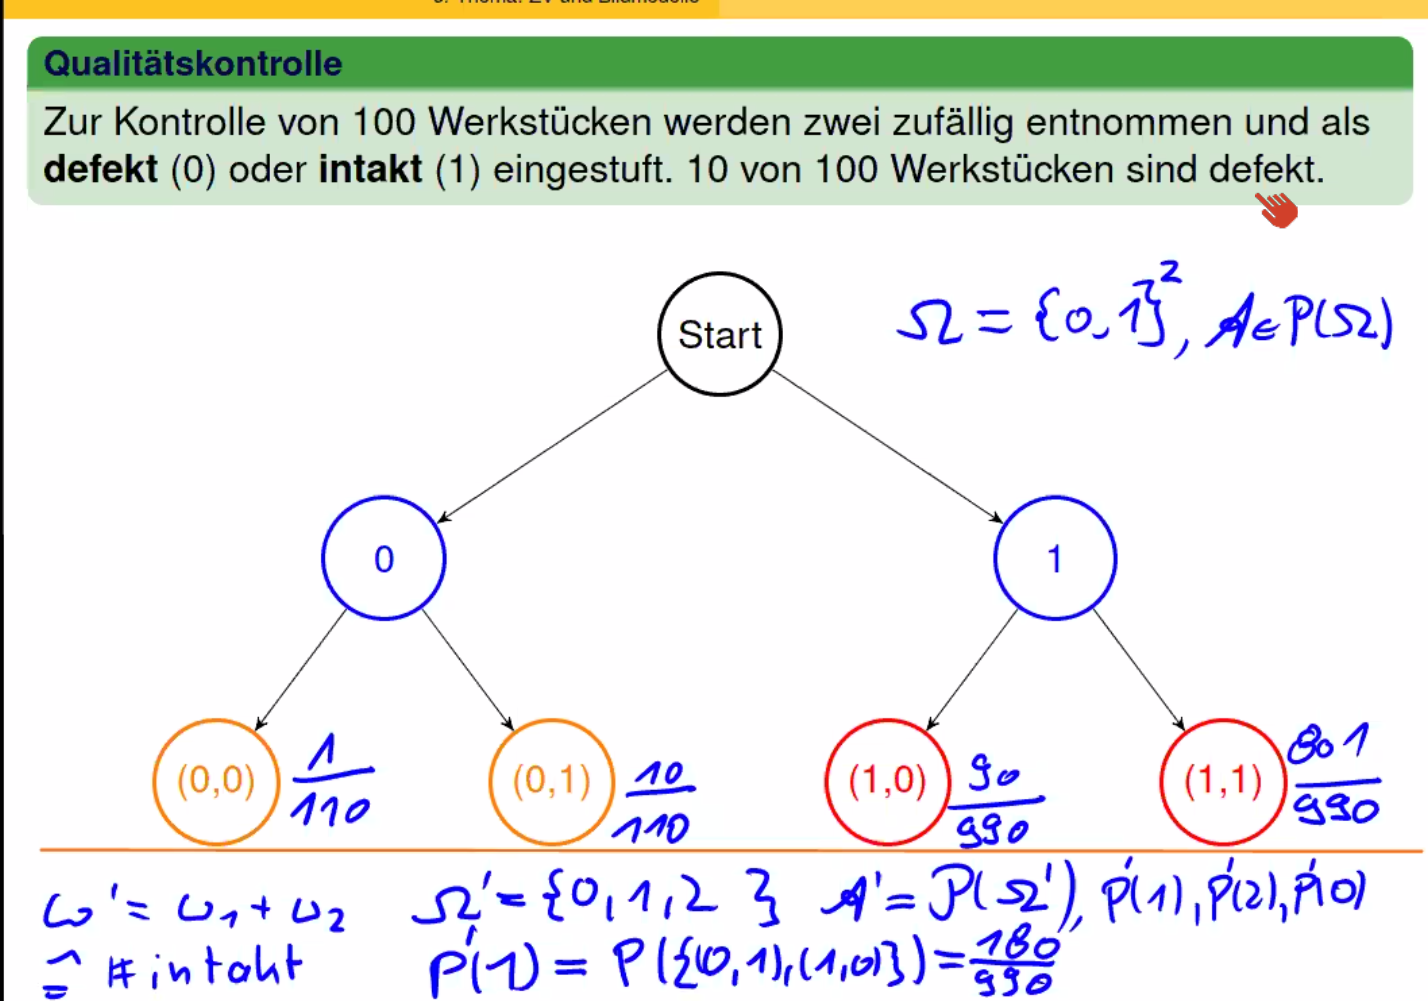
\includegraphics[height=6cm]{Urne.png}\\
	$\omega' = \omega_1+\omega_2$ $\Omega' =\{0,1,2\}$ $\mathcal{A} = \mathcal{P}(\Omega)$ $P'(1),P'(2), P'(0)$\\
	Das ist eine davon ableitbare Wahrscheinlichkeitsverteilung, wo nur die Anzahl, aber nicht die Reihenfolge wichtig sind.\\
	$\#$ intakte $P(1) = P(\{(0,1),(1,0)\}) = P(\{(0,1)\})+P(\{(1,0)\}) =\frac{10}{110} +\frac{90}{990}= \frac{180}{990}$\\
	\begin{tabular}{c|c}
	$\Omega=\{0,1\}^3,\mathcal{A} =\mathcal{P}(\Omega)$&$\Omega'=\{0,1,2\},\mathcal{A}'=\mathcal{P}(\Omega')$\\
	$P(\omega_i)=p_i$&
	\end{tabular}
	$X: (\omega_1,\omega_2)\mapsto \omega_1+\omega_2= \omega'$\\
	\includegraphics[height=6cm]{qualitätskontrolle.png}\\
	N Objekte, davon sind K markiert, weiterhin n ziehungen.\\
	W-Modell für Fertigungsprotokoll $\Omega=\{0,1\}^n$\\
	$f(\omega_1,\dots,\omega_n) = \frac{(K)_{\Sigma\omega_i} (N-K)_{n-\Sigma\omega_i}}{(N)_n}$\\
	man hat also $\binom{K}{k}$ möglichkeiten die K markierten zu ziehen.\\
	Weiterhin hat man aber $\binom{N-K}{n-k}$ nicht markierte objekte zu ziehen.\\
	Das ist im verhältnis dazu, wie viele objekte man überhaupt in n schritten ziehen kann.\\
	$$h(N,K,n;k) = \frac{\binom{K}{k}\binom{N-K}{n-k}}{\binom{N}{n}}$$
	dies ist die hypergeometrische Verteilung. (sprich was ist die wahrscheinlichkeit aus N elementen mit K Zieln in n zügen k treffer zu bekommen)\\
	$B_k = \{\text{Es werden k stücke gezogen}\}: B_k =\{Z_n=k\}$\\
	Z-Dichte:
	\[f(k)=P'(\{k\}) = P(\{Z_n=k\})=\frac{\binom{K}{k}\binom{N-K}{n-k}}{\binom{N}{n}}\]
	1.\\
	Bildmodell unter Zufallsvariable X definiert/konstruiert\\
	Ein Bildmodell wird definiert durch das Maß der darunterliegenden messbaren menge:\\
	Wenn X die zufallsvariable ist, die von $\Omega$ in das Ereignis $A'$ abbildet (es beschreibt)
	\[\{X\in A'\} = \{\omega_i\in\Omega: X(\omega_i)\in A'\}\]
	Dann definiert $X^{-1}$ die Urbildfunktion, die wieder zurück auf das Urbild abbildet:\\
	Die Wahrscheinlichkeit eines durch X beschriebenen Ereignisses, kann somit auf die Wahrscheinlichkeit der darunterliegenden Ereignisse gemapped werden:\\
	\[A'\to P^X (A'):= P(x^{-1}(A')) = P(X\in A') = P(\{\omega_i\in\Omega: X(\omega_i)\in A'\}) = \sum_{\omega_i\in\Omega: X(\omega_i)\in A'} P(\omega_i)\]
	2.\\
	Unter welchen Vorraussetzungen ist eine Approximation der Binomialverteilung durch die Poisson-.Verteilung sinnvoll:\\
	Viele Messwerte und kleine Wahrscheinlichkeiten\\
	Sei $S_n$ eine Folge von binom. Zufallsvariablen mit Parameter $n\in\mathbb{N}$ und $p_n$ und $\mathbb{E}(S_n) = n\cdot p_n\to \lambda >0$ für $n\to\infty$, dann folgt\\
	$P(S_n=k)= B(n,p_n,k) \to \frac{\lambda^k}{k!} e^{-\lambda} = P_\lambda(k)$\\
	\begin{align}\lim_{n\to\infty}P(S_n=k) & = \lim_{n\to\infty}\frac{n!}{k!\,(n-k)!}p^{k}\left(1-p\right)^{n-k}\\
	\text{subst: }p=\frac{\lambda}{n}\implies&  \lim_{n\to\infty}\frac{n!}{k!\,(n-k)!}\left(\frac{\lambda}{n}\right)^{k}\left(1-\frac{\lambda}{n}\right)^{n-k}\\
	 & =\lim_{n\to\infty}\left(\frac{\lambda^{k}}{k!}\right)\left(\frac{n(n-1)(n-2)\cdots(n-k+1)}{n^{k}}\right)\left(1-\frac{\lambda}{n}\right)^{n}\left(1-\frac{\lambda}{n}\right)^{-k}\\
	 & =\frac{\lambda^{k}}{k!}\cdot\lim_{n\to\infty}\underbrace{\left(\frac{n}{n}\cdot\frac{n-1}{n}\cdot\frac{n-2}{n}\cdots\frac{n-k+1}{n}\right)}_{\to1}\underbrace{\left(1-\frac{\lambda}{n}\right)^{n}}_{\to e^{-\lambda}}\underbrace{\left(1-\frac{\lambda}{n}\right)^{-k}}_{\to1}\\
	 & =\frac{\lambda^{k}\mathrm{e}^{-\lambda}}{k!}.
	 \end{align}
	Man kann hieran sehen, dass wenn n sehr groß ist, oder p sehr klein (weil p als $\frac{\lambda}{n}$ dargestellt wird) ist.\\
	3. Aussage des Zentralen Grenzwertsatzes:\\
	Wenn man sehr viele kleiner unabhängiger Zufallseffekte $n\to\infty$ und kleine Wahrscheinlichkeiten hat $p<<1$ dann kann eine Verteilung als eine Normalverteilung modelliert werden, solange keine einzelne Variable einen dominanten einfluss auf die Varianz besitzt.\\
	Beweis: n i.i.d Zufallsvariablen $X_1,X_2,\dots$: Erwartungswert $\mu$ und std $\sigma$.\\
	$S_n = X_1+X_2+\dots+X_n$ Der Erwartungswert ist $n\mu$ und Var $n\sigma^2$. Standardisieren:\\
	$Z_n = \frac{S_n-n\mu}{\sigma\sqrt{n}}$.\\
	Der zentrale Grenzwertsatz besagt, dass $Z_n$ für $n\to\infty$ zur standardnormalverteilung punktweise konvergiert $\mathcal{N}(0,1)$\\
	Faustregel für anpassung von Normalverteilung an Binomialverteilung.\\
	$n\cdot p\cdot (1-p)\geq 9$ und $np\geq 5$, dann $\mathcal{N}(np, np(1-p))$\\
\end{document}